\documentclass{article}\usepackage[]{graphicx}\usepackage[]{color}
% maxwidth is the original width if it is less than linewidth
% otherwise use linewidth (to make sure the graphics do not exceed the margin)
\makeatletter
\def\maxwidth{ %
  \ifdim\Gin@nat@width>\linewidth
    \linewidth
  \else
    \Gin@nat@width
  \fi
}
\makeatother

\definecolor{fgcolor}{rgb}{0.345, 0.345, 0.345}
\newcommand{\hlnum}[1]{\textcolor[rgb]{0.686,0.059,0.569}{#1}}%
\newcommand{\hlstr}[1]{\textcolor[rgb]{0.192,0.494,0.8}{#1}}%
\newcommand{\hlcom}[1]{\textcolor[rgb]{0.678,0.584,0.686}{\textit{#1}}}%
\newcommand{\hlopt}[1]{\textcolor[rgb]{0,0,0}{#1}}%
\newcommand{\hlstd}[1]{\textcolor[rgb]{0.345,0.345,0.345}{#1}}%
\newcommand{\hlkwa}[1]{\textcolor[rgb]{0.161,0.373,0.58}{\textbf{#1}}}%
\newcommand{\hlkwb}[1]{\textcolor[rgb]{0.69,0.353,0.396}{#1}}%
\newcommand{\hlkwc}[1]{\textcolor[rgb]{0.333,0.667,0.333}{#1}}%
\newcommand{\hlkwd}[1]{\textcolor[rgb]{0.737,0.353,0.396}{\textbf{#1}}}%
\let\hlipl\hlkwb

\usepackage{framed}
\makeatletter
\newenvironment{kframe}{%
 \def\at@end@of@kframe{}%
 \ifinner\ifhmode%
  \def\at@end@of@kframe{\end{minipage}}%
  \begin{minipage}{\columnwidth}%
 \fi\fi%
 \def\FrameCommand##1{\hskip\@totalleftmargin \hskip-\fboxsep
 \colorbox{shadecolor}{##1}\hskip-\fboxsep
     % There is no \\@totalrightmargin, so:
     \hskip-\linewidth \hskip-\@totalleftmargin \hskip\columnwidth}%
 \MakeFramed {\advance\hsize-\width
   \@totalleftmargin\z@ \linewidth\hsize
   \@setminipage}}%
 {\par\unskip\endMakeFramed%
 \at@end@of@kframe}
\makeatother

\definecolor{shadecolor}{rgb}{.97, .97, .97}
\definecolor{messagecolor}{rgb}{0, 0, 0}
\definecolor{warningcolor}{rgb}{1, 0, 1}
\definecolor{errorcolor}{rgb}{1, 0, 0}
\newenvironment{knitrout}{}{} % an empty environment to be redefined in TeX

\usepackage{alltt}

\usepackage{float}

% Set the margins on the page to not be so large
\addtolength{\oddsidemargin}{-.875in}
\addtolength{\evensidemargin}{-.875in}
\addtolength{\textwidth}{1.75in}
\addtolength{\topmargin}{-.875in}
\addtolength{\textheight}{1.75in}

% Take off page numbering
\pagenumbering{gobble}
\IfFileExists{upquote.sty}{\usepackage{upquote}}{}
\begin{document}

\title{%
  2.2.2: R - Linear Regression Remedial Measures\\
  \smallskip
  \large Stat 5100: Dr. Bean
}
\date{}

\maketitle

\textbf{Example: } Age and plasma levels for 25 healthy children in a study are reported. Of interest is how plasma level depends on age.

\begin{knitrout}
\definecolor{shadecolor}{rgb}{0.969, 0.969, 0.969}\color{fgcolor}\begin{kframe}
\begin{alltt}
\hlcom{# Load data}
\hlkwd{library}\hlstd{(stat5100)}
\hlkwd{data}\hlstd{(plasma)}

\hlcom{# Fit regression model and check assumptions}
\hlstd{plasma_lm} \hlkwb{<-} \hlkwd{lm}\hlstd{(level} \hlopt{~} \hlstd{age,} \hlkwc{data} \hlstd{= plasma)}

\hlcom{# Check visual assumptions}
\hlcom{# (Note: this is a new function you haven't seen before, all this one does}
\hlcom{# is it combines the work from seq_plot, qq_plot, residual_hist, and}
\hlcom{# residual_plot into one single image)}
\hlkwd{visual_assumptions}\hlstd{(plasma_lm)}
\end{alltt}
\end{kframe}
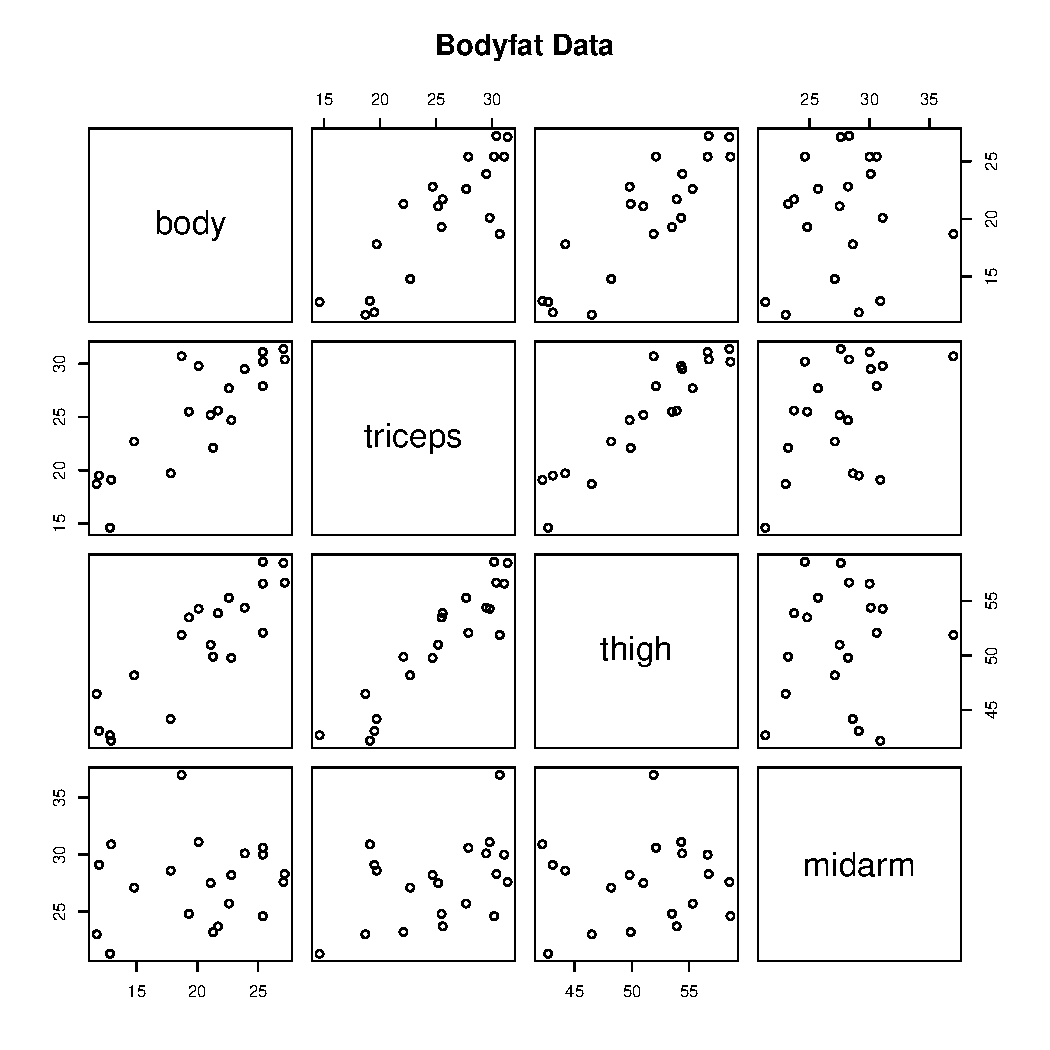
\includegraphics[width=0.6\textwidth]{figure/unnamed-chunk-1-1} 
\begin{kframe}\begin{alltt}
\hlcom{# Check assumptions with numerical tests}
\hlkwd{brown_forsythe_lm}\hlstd{(plasma_lm)}
\end{alltt}
\begin{verbatim}
## [1] "Brown-forsythe test for constant variance in the residuals:"
## [1] "T-statistic: -1.6903, p-value: 0.1045"
\end{verbatim}
\begin{alltt}
\hlkwd{cor_normality_lm}\hlstd{(plasma_lm)}
\end{alltt}
\begin{verbatim}
## Correlation test of normality:
##                   resid expected_norm
## resid         1.0000000     0.9036011
## expected_norm 0.9036011     1.0000000
## 
## Total observations: 25
## Make sure to consult with table B.6 for your final result.
\end{verbatim}
\begin{alltt}
\hlkwd{ftest_lackfit_lm}\hlstd{(plasma_lm)}
\end{alltt}
\begin{verbatim}
## Analysis of Variance Table
## 
## Model 1: level ~ age
## Model 2: level ~ age
##   Res.Df    RSS Df Sum of Sq      F  Pr(>F)  
## 1     23 77.983                              
## 2     20 55.234  3    22.749 2.7457 0.06994 .
## ---
## Signif. codes:  0 '***' 0.001 '**' 0.01 '*' 0.05 '.' 0.1 ' ' 1
\end{verbatim}
\begin{alltt}
\hlcom{# Consider transformations}
\hlkwd{library}\hlstd{(MASS)}
\hlkwd{boxcox}\hlstd{(level} \hlopt{~} \hlstd{age,} \hlkwc{data} \hlstd{= plasma)}
\end{alltt}
\end{kframe}
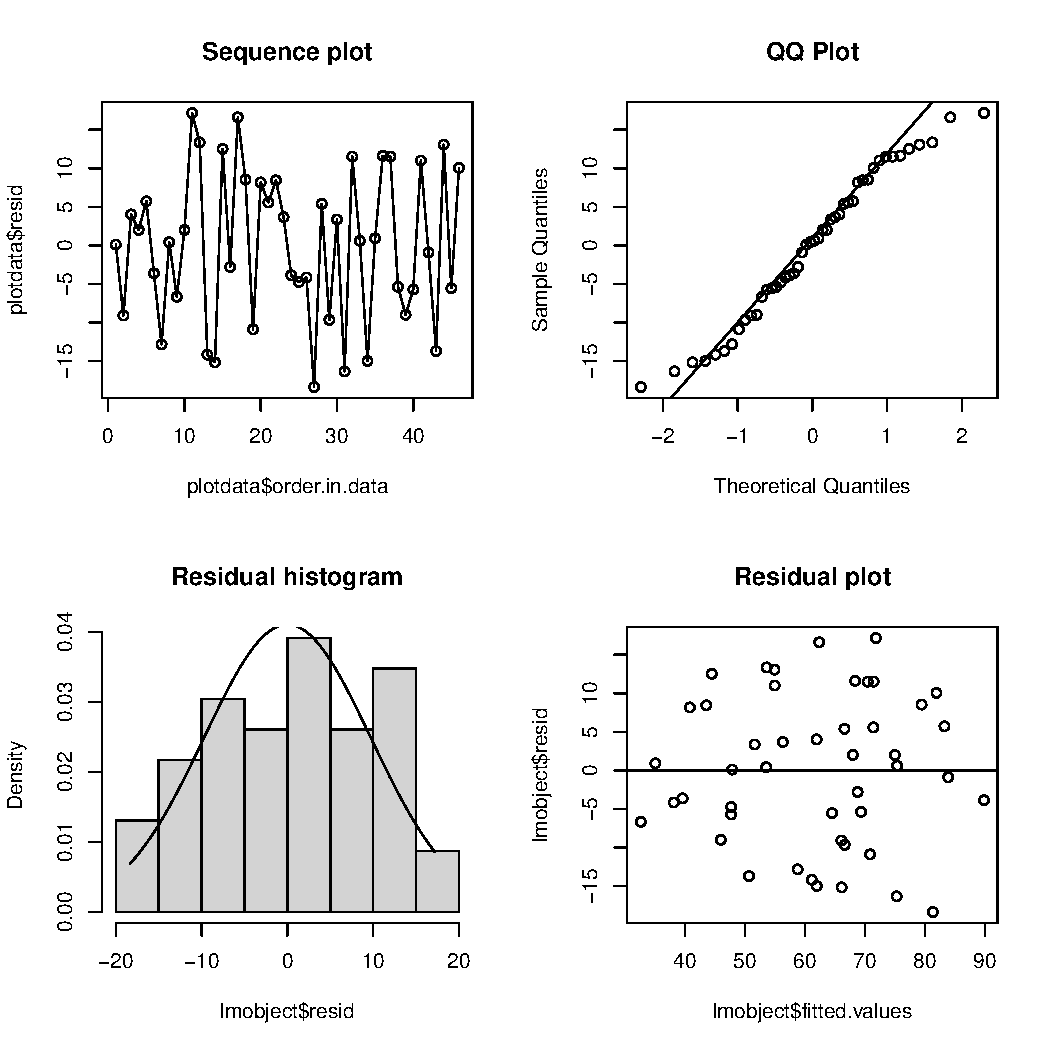
\includegraphics[width=0.6\textwidth]{figure/unnamed-chunk-1-2} 
\begin{kframe}\begin{alltt}
\hlcom{# The above plot tells us we could consider either a log transform or}
\hlcom{# possible a 1/(sqrt(response)) type of transform. We will try both and}
\hlcom{# show the new visual checks for model assumptions for each.}
\hlstd{plasma} \hlkwb{<-} \hlkwd{cbind}\hlstd{(plasma,} \hlkwc{log_level} \hlstd{=} \hlkwd{log}\hlstd{(plasma}\hlopt{$}\hlstd{level),}
                \hlkwc{invsqrt_level} \hlstd{=} \hlnum{1} \hlopt{/} \hlkwd{sqrt}\hlstd{(plasma}\hlopt{$}\hlstd{level))}

\hlcom{# LOG TRANSFORM}
\hlcom{# ---------------}

\hlstd{plasma_log_lm} \hlkwb{<-} \hlkwd{lm}\hlstd{(log_level} \hlopt{~} \hlstd{age,} \hlkwc{data} \hlstd{= plasma)}
\hlkwd{visual_assumptions}\hlstd{(plasma_log_lm)}
\end{alltt}
\end{kframe}
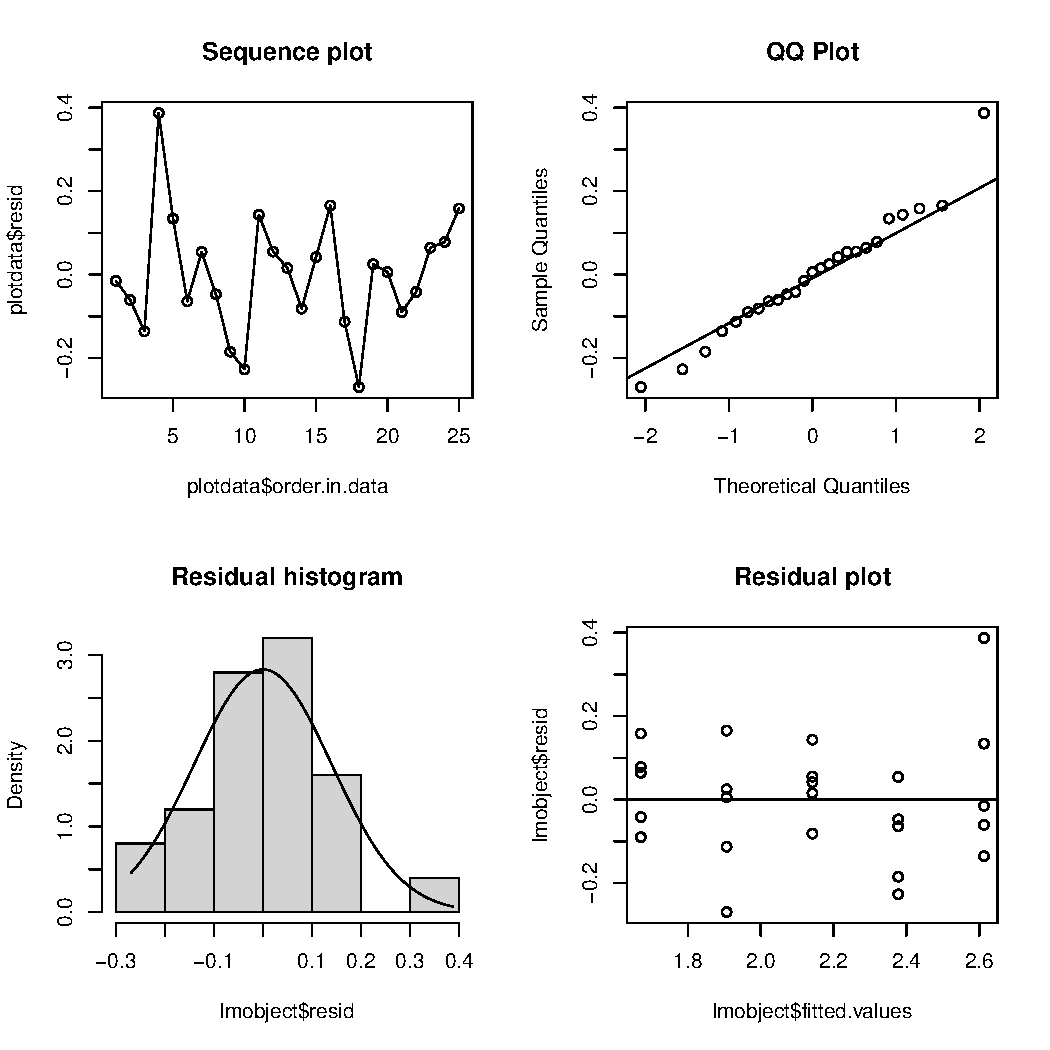
\includegraphics[width=0.6\textwidth]{figure/unnamed-chunk-1-3} 
\begin{kframe}\begin{alltt}
\hlcom{# Numerical checks}
\hlkwd{brown_forsythe_lm}\hlstd{(plasma_log_lm)}
\end{alltt}
\begin{verbatim}
## [1] "Brown-forsythe test for constant variance in the residuals:"
## [1] "T-statistic: -0.7958, p-value: 0.4343"
\end{verbatim}
\begin{alltt}
\hlkwd{cor_normality_lm}\hlstd{(plasma_log_lm)}
\end{alltt}
\begin{verbatim}
## Correlation test of normality:
##                   resid expected_norm
## resid         1.0000000     0.9807112
## expected_norm 0.9807112     1.0000000
## 
## Total observations: 25
## Make sure to consult with table B.6 for your final result.
\end{verbatim}
\begin{alltt}
\hlcom{# INVERSE SQUARE ROOT TRANSFORM}
\hlcom{# ------------------------------}

\hlstd{plasma_invsqrt_lm} \hlkwb{<-} \hlkwd{lm}\hlstd{(invsqrt_level} \hlopt{~} \hlstd{age,} \hlkwc{data} \hlstd{= plasma)}
\hlkwd{visual_assumptions}\hlstd{(plasma_invsqrt_lm)}
\end{alltt}
\end{kframe}
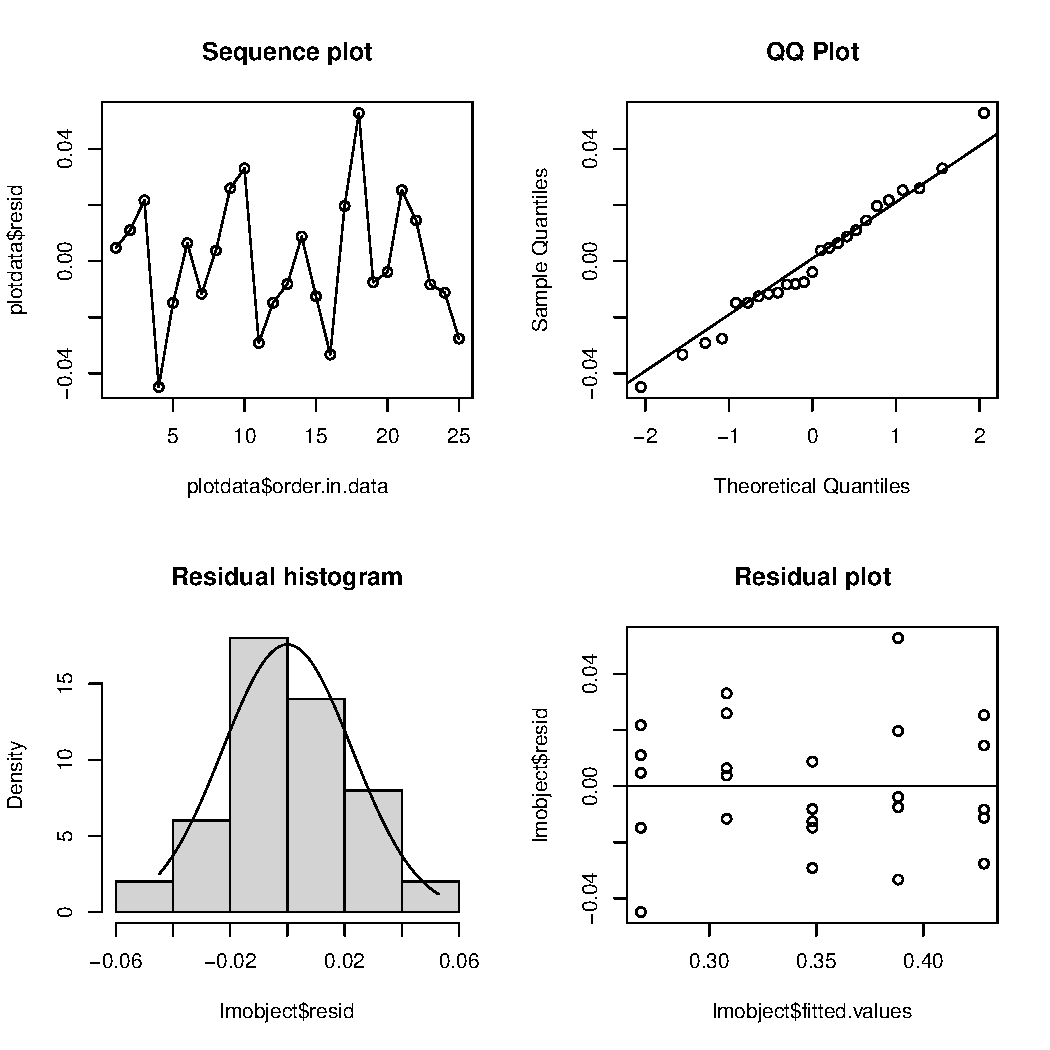
\includegraphics[width=0.6\textwidth]{figure/unnamed-chunk-1-4} 
\begin{kframe}\begin{alltt}
\hlcom{# Numerical checks}
\hlkwd{brown_forsythe_lm}\hlstd{(plasma_invsqrt_lm)}
\end{alltt}
\begin{verbatim}
## [1] "Brown-forsythe test for constant variance in the residuals:"
## [1] "T-statistic: -0.5031, p-value: 0.6197"
\end{verbatim}
\begin{alltt}
\hlkwd{cor_normality_lm}\hlstd{(plasma_invsqrt_lm)}
\end{alltt}
\begin{verbatim}
## Correlation test of normality:
##                   resid expected_norm
## resid         1.0000000     0.9918794
## expected_norm 0.9918794     1.0000000
## 
## Total observations: 25
## Make sure to consult with table B.6 for your final result.
\end{verbatim}
\end{kframe}
\end{knitrout}


\end{document}
